\section{Results} \label{sec:results}

\todo[inline,author=Pedro]{This section will present and discuss the results,
connecting the findings with normalization techniques and problem domains.}

\subsection{Travelling Salesperson Problem}

\todo[inline,author=Pedro]{Here we will discuss the results for the TSP. We
will argue that we achieved results very close to a high-end machine
using cheap and low-end virtual machines.}

\begin{figure}[htpb]
    \centering
    \begin{minipage}{.45\textwidth}
        \centering
        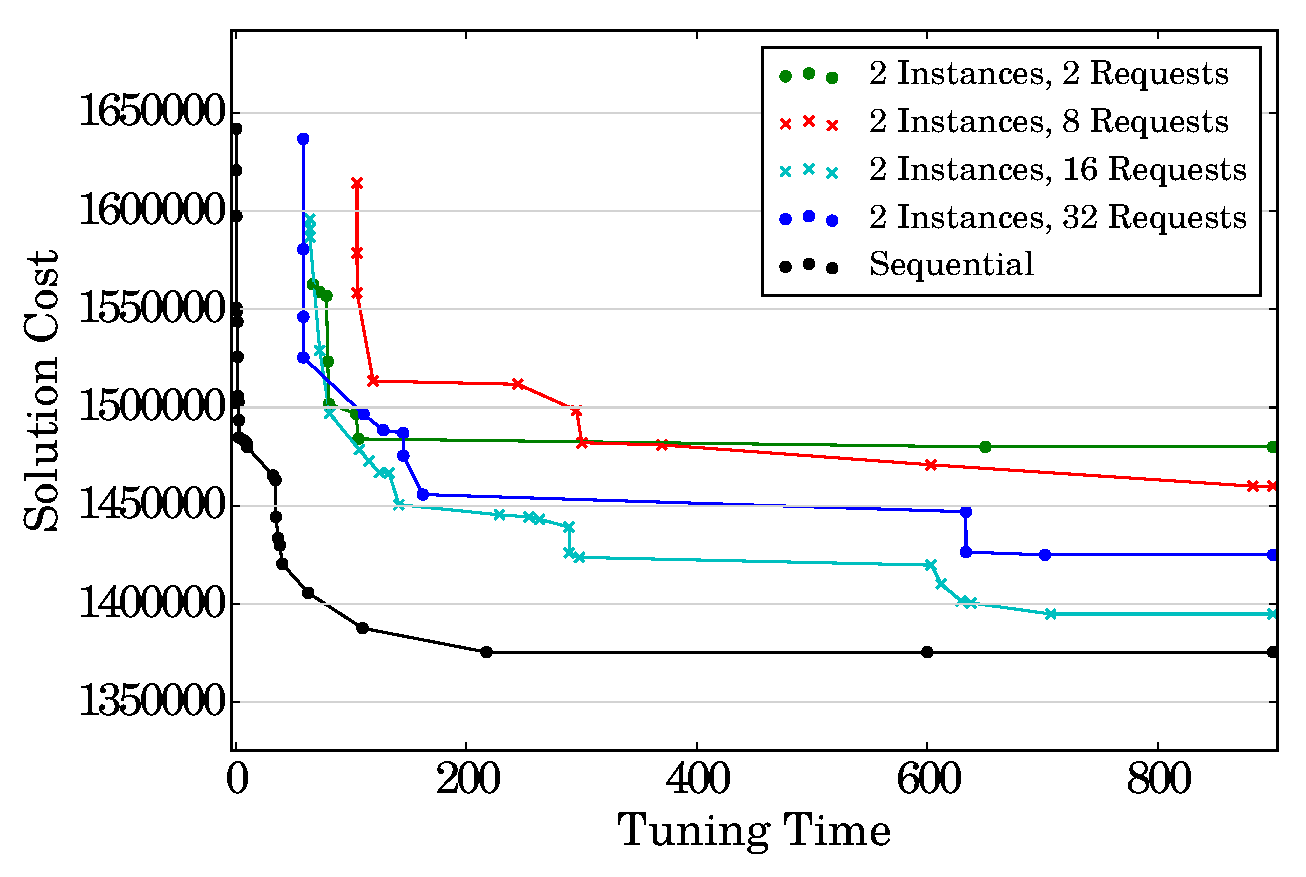
\includegraphics[scale=.35]{i2_p_n_comparison}
        \caption{Measurements using two virtual machine instances, solving
                 a TSP instance of size 532.}
        \label{fig:high-level}
    \end{minipage}%
    \hfill
    \begin{minipage}{.45\textwidth}
        \centering
        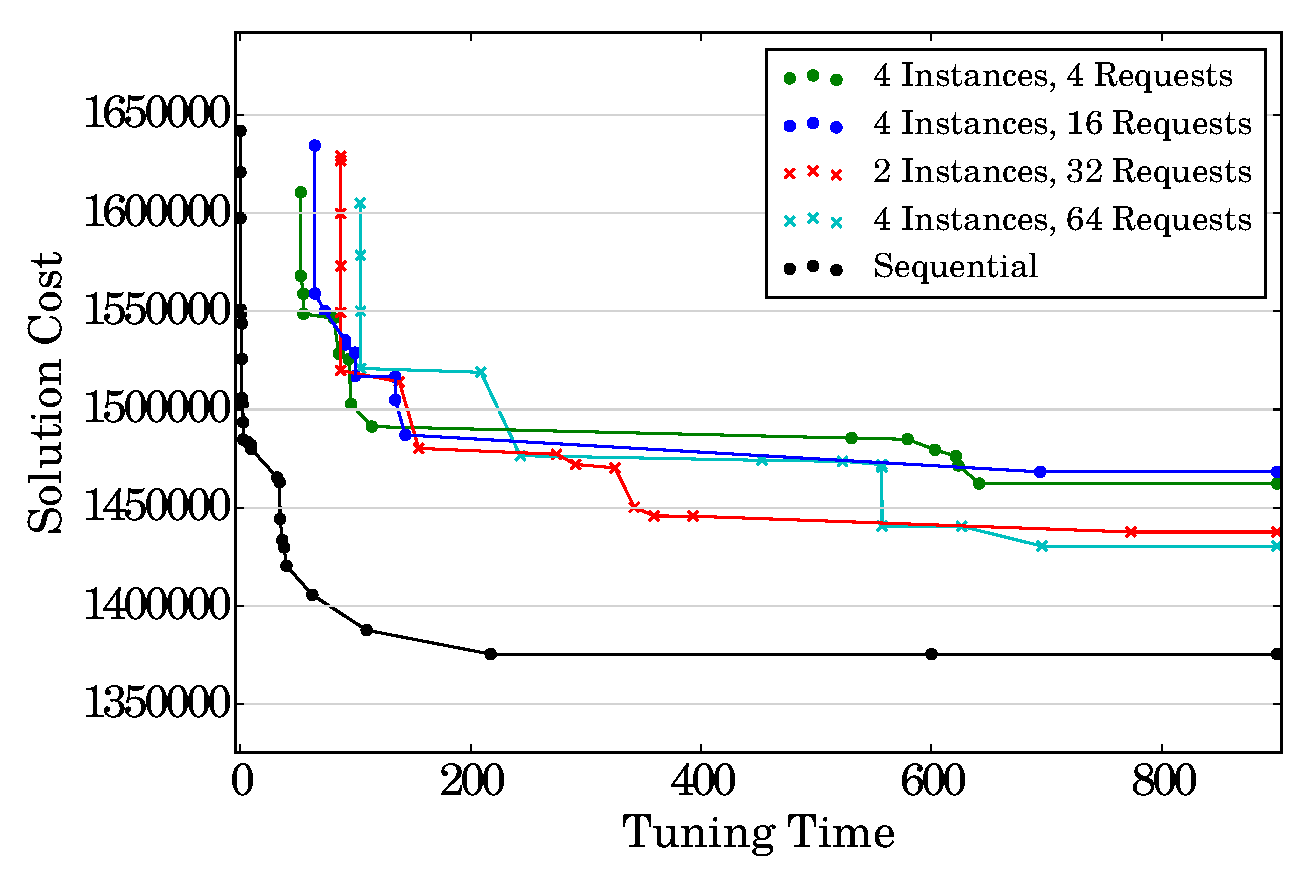
\includegraphics[scale=.35]{i4_p_n_comparison}
        \caption{Measurements using four virtual machine instances,
                 solving a TSP instance of size 532.}
        \label{fig:low-level}
    \end{minipage}%
    \label{fig:archs}
\end{figure}

\begin{figure}[htpb]
    \centering
    \begin{minipage}{.45\textwidth}
        \centering
        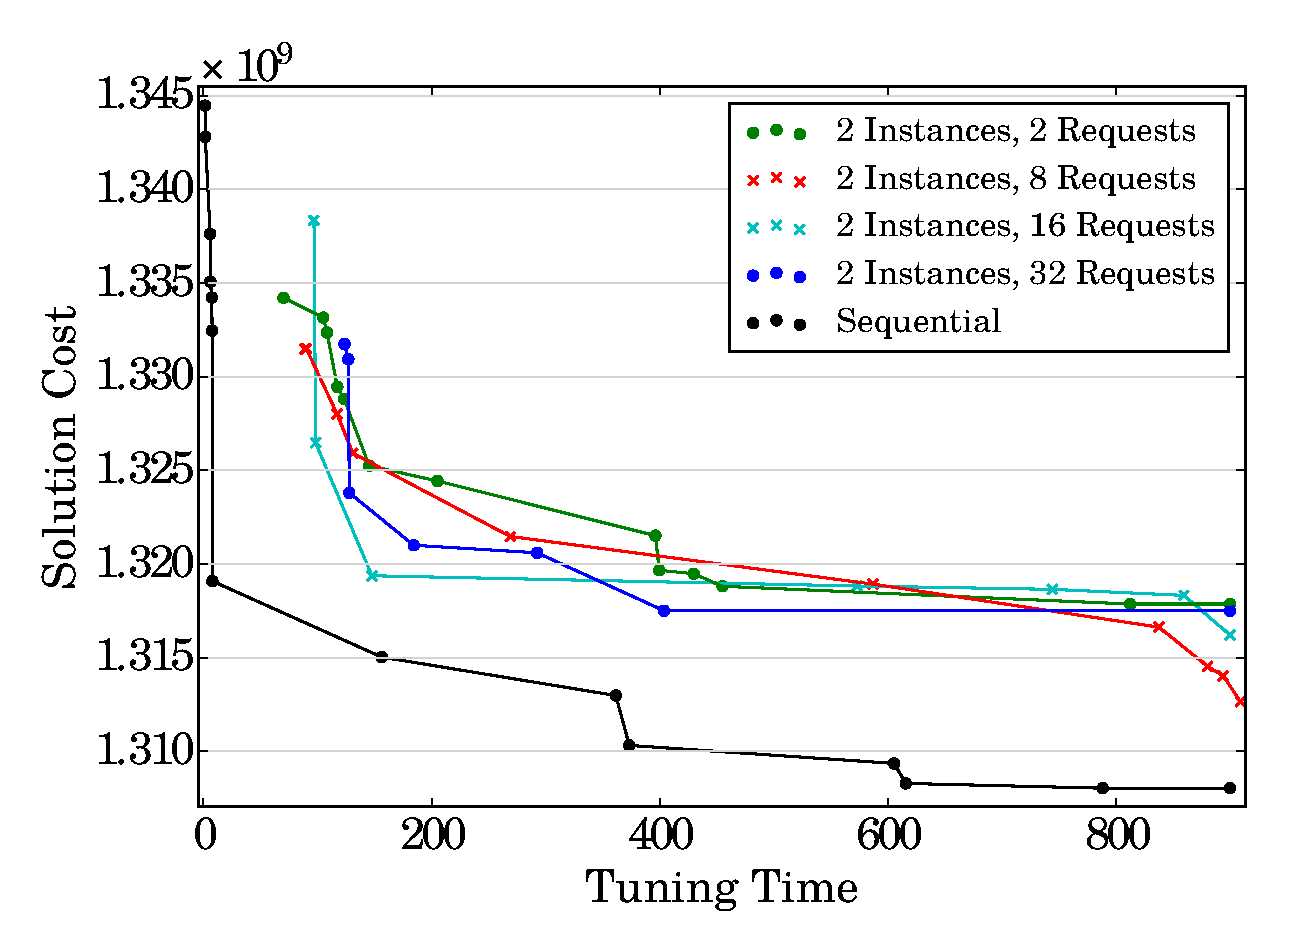
\includegraphics[scale=.35]{i2_p_n_comparison_85900}
        \caption{Measurements using two virtual machine instances,
                 solving an instance of size 85900.}
        \label{fig:high-level}
    \end{minipage}%
    \hfill
    \begin{minipage}{.45\textwidth}
        \centering
        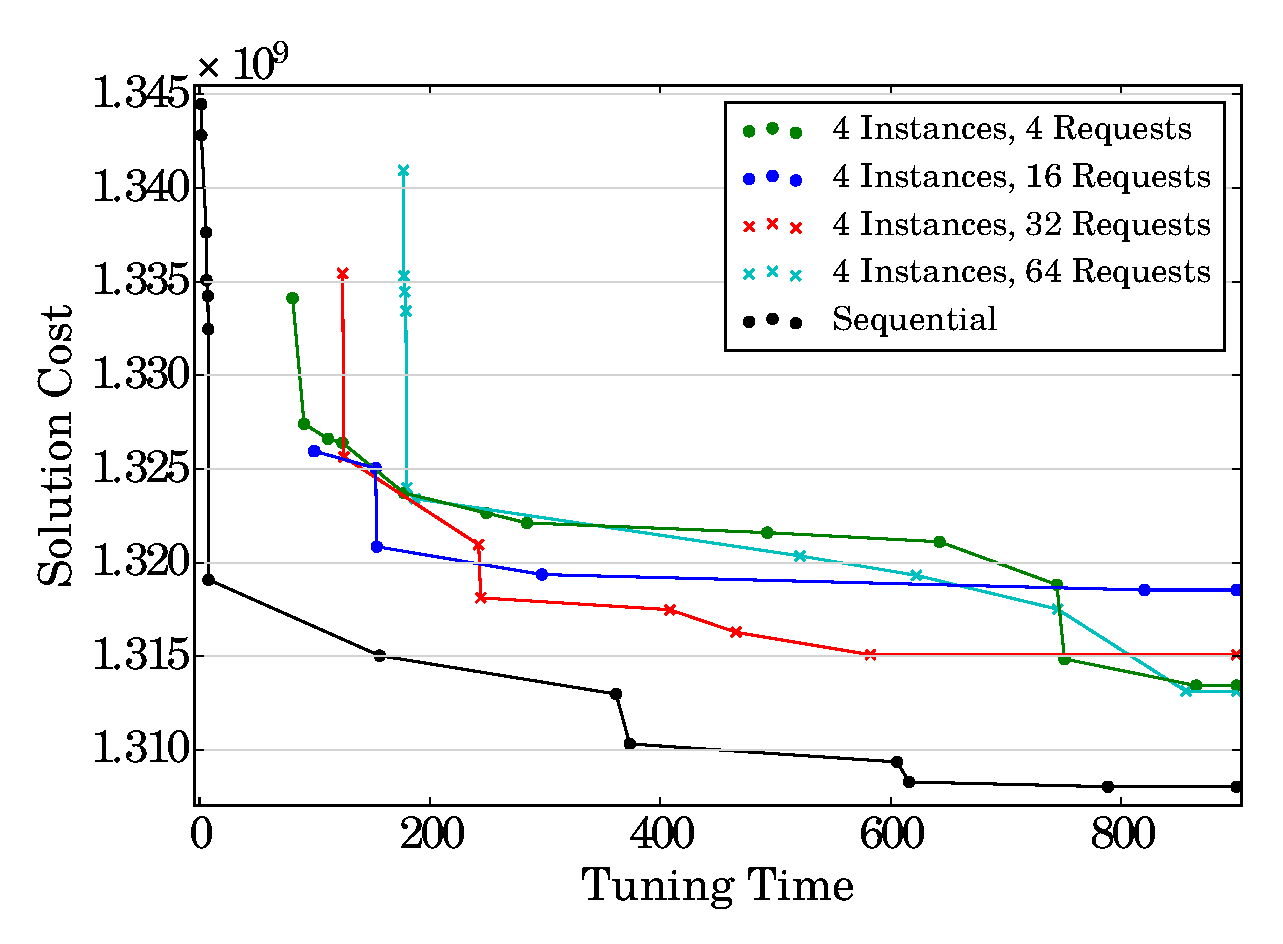
\includegraphics[scale=.35]{i4_p_n_comparison_85900}
        \caption{Measurements using four virtual machine instances,
                 solving an instance of size 85900.}
        \label{fig:low-level}
    \end{minipage}%
    \label{fig:archs}
\end{figure}
